\chapter{Urinveier}%urinveiene
		\section{Gullkornene:}
			\begin{itemize}
				\item Vanligere med urinveisinfeksjon i høyere alder.\\
				\item En vanlig årsak til delir(se side \pageref{delir}).\\
				\item Bakterier i urinen til gamle damer behøver ikke være farlig.\\
				\item Lukt og farge kan lure oss.\\
			\end{itemize}
		\section{Anatomi}
					\begin{figure}[ht]
                      \centering
                      	\frame{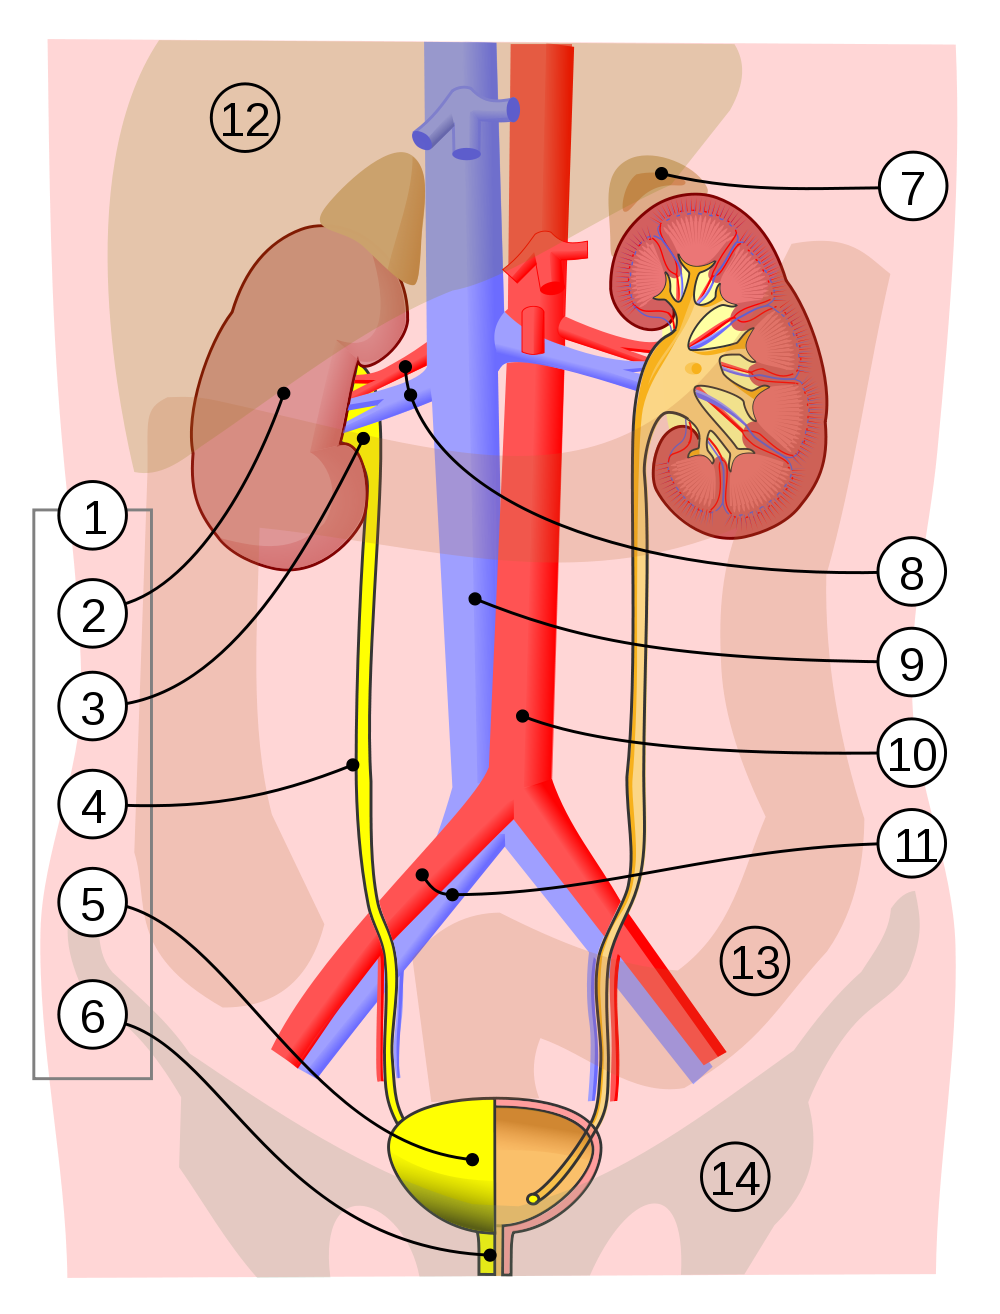
\includegraphics[width=5in]{./kap/bilder/urinveier.png}}%!!! må byttes ut, copyright Greys anatomy
                      \caption{\emph{1.} Urinveiene ,\emph{2.} Nyre, \emph{3.} Nyrebekkenet, \emph{4.} Urether, \emph{5.} Blæra, \emph{6.} Urethra, \emph{7.} Binyre, \emph{8.} Nyrearterie og -vene, \emph{9.} Vena cava inferior, \emph{10.} Bukaorta, \emph{11.} Arteria og Vena Iliaca, \emph{12.} Lever, \emph{13.} Tykktarmen, \emph{14.} Bekkenet}
                    \end{figure}
			\paragraph{Feilkonstruksjon?\\}
				Kvinner har et kort urinrør som gjør det svært lett å få urinveisinfeksjoner. At eldre damer har bakterier i urinen uten symptomer er forholdsvis vanlig og ikke farlig\cite{uti-old}
			\paragraph{Den svake strålen\\}
				Menn har også hyppigere infeksjoner med alderen. Det er ofte prostaten, plager etter operasjon og kateterbruk som gjør dette. 
		\section{Fysiologi}
			Bakteriene vandrer nedenfra og opp. Urin er steril hos friske. Eldre med bakterier uten symptomer trenger vanligvis ikke behandling. 
		\section{Patologi}
			\paragraph{Flere nivåer\\}
				Bakteriene irriterer lokalt og skaper smerter når man er på do. Noen får generell slapphet av den pågående reaksjonen. Hvis bakteriene kommer opp til nyrene kalles det pyelonefritt, eller nyrebekkenbetennelse. Kommer de enda høyere kalles det urosepsis og er kjennetegnet av at bakteriene sprer seg i hele kroppen via blodet. 
		\section{Klinikk}
			\subsection{UVI}
				Veldig vanlig og trenger ikke behandling dersom fravær av symptomer. Pasienten bør følges tett dersom bakterier påvises, for deretter å kunne slippe opp litt. Man i disse pasientene huske på at urinveiene an være årsak ved sykdom. Ta urinprøver regelmessig, men det behøver ikke føre til behandling.
		\section{Pasienteksempler}
			\subsection{Pasient 7}
			\subsection{Pasient 8}